\documentclass{standalone}
\usepackage{tikz}
\usetikzlibrary{patterns}
\usetikzlibrary{positioning}
\usetikzlibrary{patterns, positioning}
\usetikzlibrary{shapes.misc}
\usepackage[outline]{contour}
\contourlength{1.5pt} 
\usepackage[sfdefault]{ClearSans}

\begin{document}
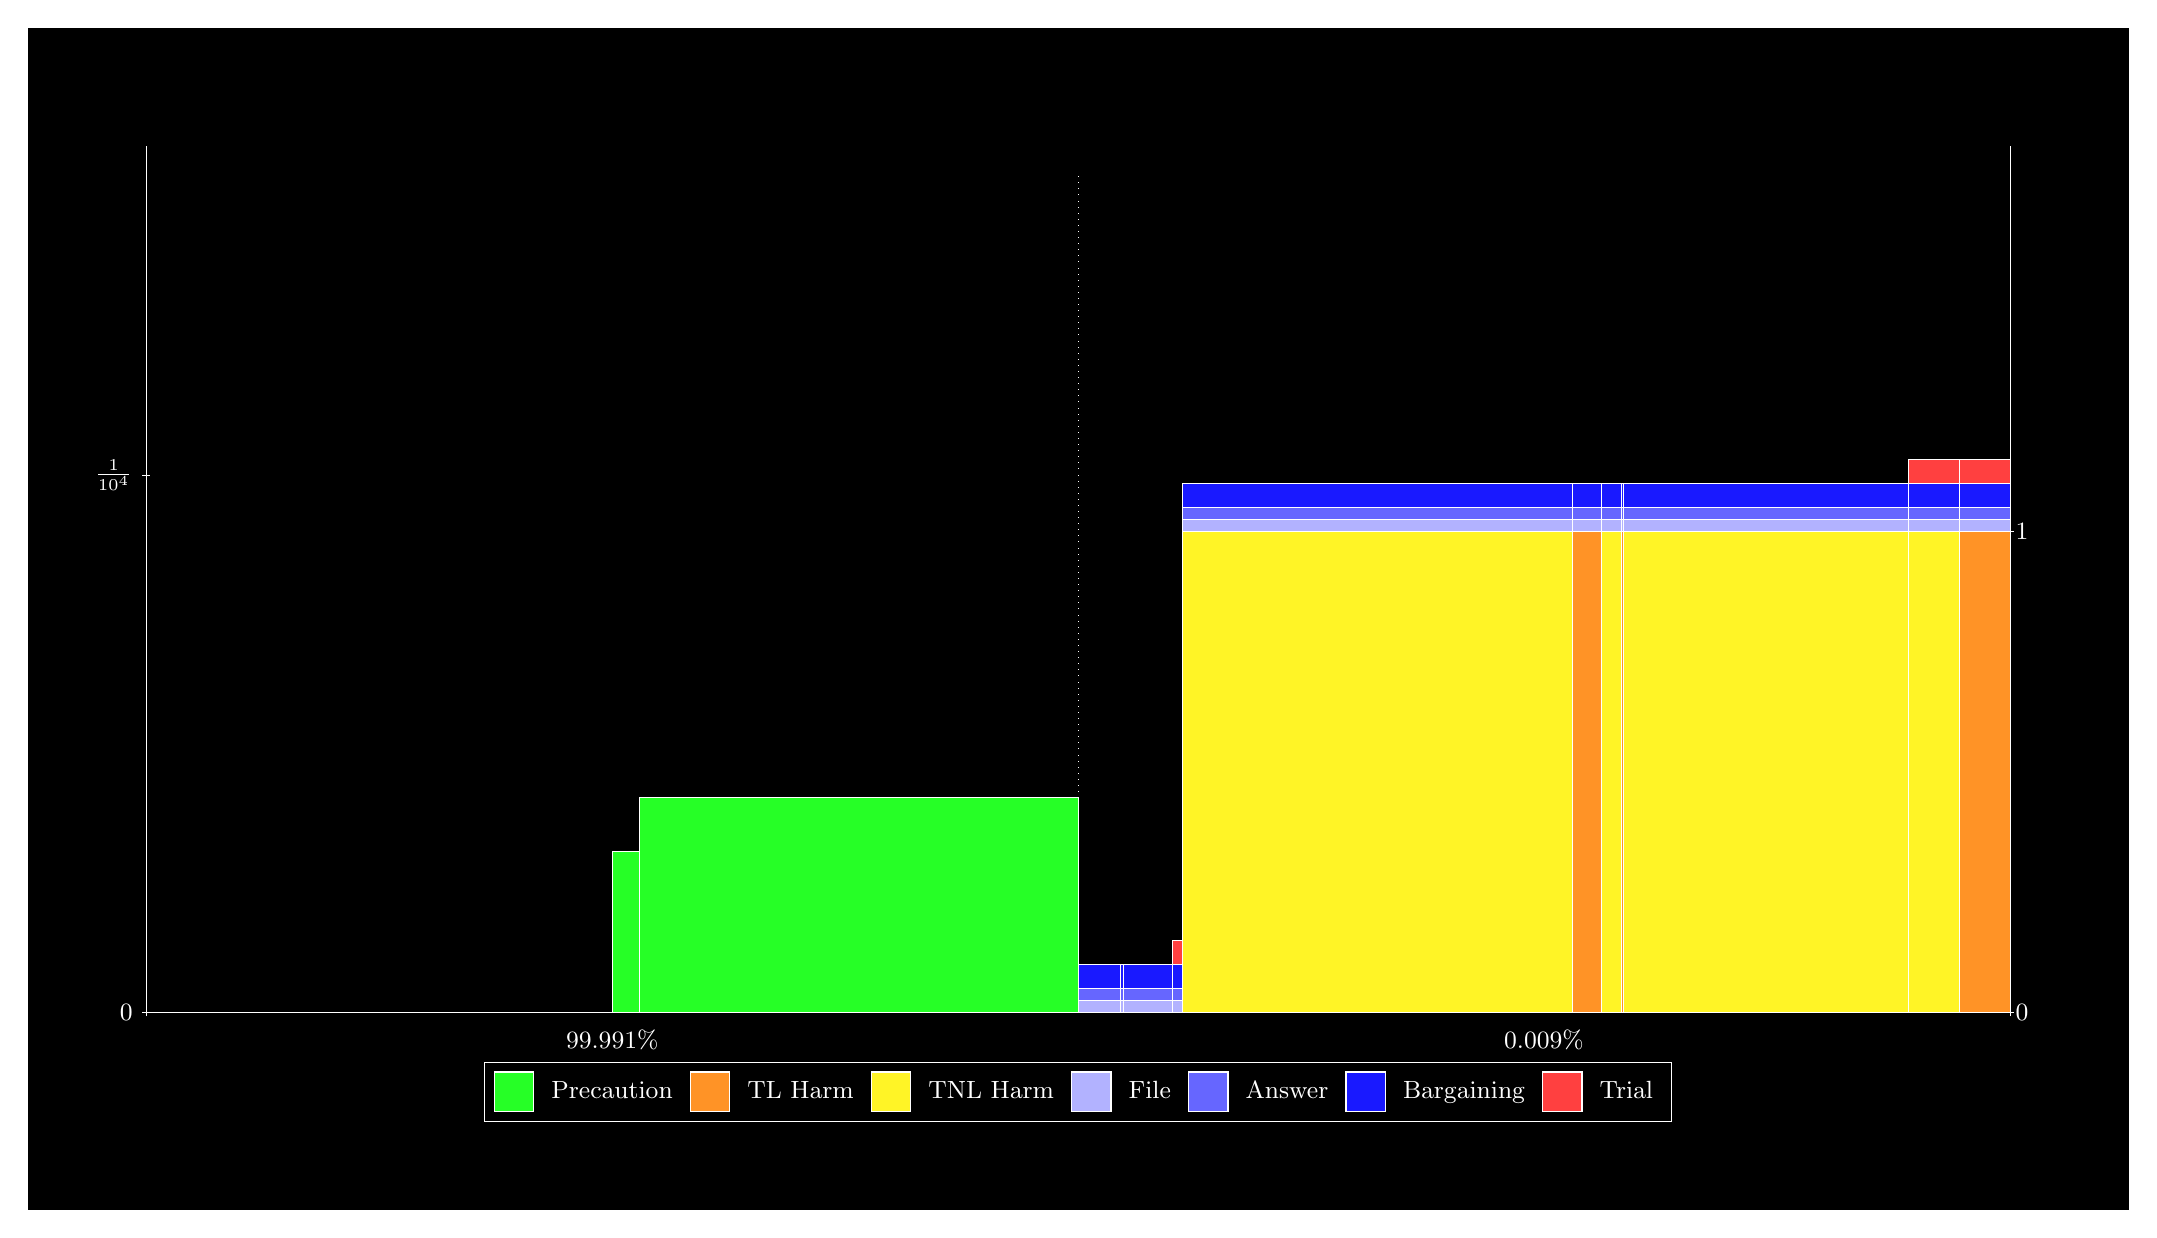
\begin{tikzpicture}
\draw[fill=black] (0,0) rectangle (26.667,15);
\draw[fill=green!85,draw=white,very thin] (7.4165,2.5) rectangle (7.7562,4.5472);
\draw[fill=green!85,draw=white,very thin] (7.7562,2.5) rectangle (13.333,5.2296);
\draw[fill=blue!30,draw=white,very thin] (13.333,2.5) rectangle (13.866,2.6527);
\draw[fill=blue!60,draw=white,very thin] (13.333,2.6527) rectangle (13.866,2.8055);
\draw[fill=blue!90,draw=white,very thin] (13.333,2.8055) rectangle (13.866,3.111);
\draw[fill=green!85,draw=white,very thin] (13.866,2.5) rectangle (13.904,2.5002);
\draw[fill=blue!30,draw=white,very thin] (13.866,2.5002) rectangle (13.904,2.6529);
\draw[fill=blue!60,draw=white,very thin] (13.866,2.6529) rectangle (13.904,2.8057);
\draw[fill=blue!90,draw=white,very thin] (13.866,2.8057) rectangle (13.904,3.1112);
\draw[fill=green!85,draw=white,very thin] (13.904,2.5) rectangle (14.53,2.5002);
\draw[fill=blue!30,draw=white,very thin] (13.904,2.5002) rectangle (14.53,2.653);
\draw[fill=blue!60,draw=white,very thin] (13.904,2.653) rectangle (14.53,2.8057);
\draw[fill=blue!90,draw=white,very thin] (13.904,2.8057) rectangle (14.53,3.1112);
\draw[fill=blue!30,draw=white,very thin] (14.53,2.5) rectangle (14.659,2.6527);
\draw[fill=blue!60,draw=white,very thin] (14.53,2.6527) rectangle (14.659,2.8055);
\draw[fill=blue!90,draw=white,very thin] (14.53,2.8055) rectangle (14.659,3.111);
\draw[fill=red!75,draw=white,very thin] (14.53,3.111) rectangle (14.659,3.4165);
\draw[fill=yellow!85,draw=white,very thin] (14.659,2.5) rectangle (19.605,8.6098);
\draw[fill=blue!30,draw=white,very thin] (14.659,8.6098) rectangle (19.605,8.7626);
\draw[fill=blue!60,draw=white,very thin] (14.659,8.7626) rectangle (19.605,8.9153);
\draw[fill=blue!90,draw=white,very thin] (14.659,8.9153) rectangle (19.605,9.2208);
\draw[fill=orange!85,draw=white,very thin] (19.605,2.5) rectangle (19.983,8.6098);
\draw[fill=blue!30,draw=white,very thin] (19.605,8.6098) rectangle (19.983,8.7626);
\draw[fill=blue!60,draw=white,very thin] (19.605,8.7626) rectangle (19.983,8.9153);
\draw[fill=blue!90,draw=white,very thin] (19.605,8.9153) rectangle (19.983,9.2208);
\draw[fill=green!85,draw=white,very thin] (19.983,2.5) rectangle (20.234,2.5002);
\draw[fill=yellow!85,draw=white,very thin] (19.983,2.5002) rectangle (20.234,8.61);
\draw[fill=blue!30,draw=white,very thin] (19.983,8.61) rectangle (20.234,8.7627);
\draw[fill=blue!60,draw=white,very thin] (19.983,8.7627) rectangle (20.234,8.9155);
\draw[fill=blue!90,draw=white,very thin] (19.983,8.9155) rectangle (20.234,9.221);
\draw[fill=green!85,draw=white,very thin] (20.234,2.5) rectangle (20.251,2.5002);
\draw[fill=orange!85,draw=white,very thin] (20.234,2.5002) rectangle (20.251,8.61);
\draw[fill=blue!30,draw=white,very thin] (20.234,8.61) rectangle (20.251,8.7627);
\draw[fill=blue!60,draw=white,very thin] (20.234,8.7627) rectangle (20.251,8.9155);
\draw[fill=blue!90,draw=white,very thin] (20.234,8.9155) rectangle (20.251,9.221);
\draw[fill=green!85,draw=white,very thin] (20.251,2.5) rectangle (23.882,2.5002);
\draw[fill=yellow!85,draw=white,very thin] (20.251,2.5002) rectangle (23.882,8.6101);
\draw[fill=blue!30,draw=white,very thin] (20.251,8.6101) rectangle (23.882,8.7628);
\draw[fill=blue!60,draw=white,very thin] (20.251,8.7628) rectangle (23.882,8.9155);
\draw[fill=blue!90,draw=white,very thin] (20.251,8.9155) rectangle (23.882,9.221);
\draw[fill=yellow!85,draw=white,very thin] (23.882,2.5) rectangle (24.525,8.6098);
\draw[fill=blue!30,draw=white,very thin] (23.882,8.6098) rectangle (24.525,8.7626);
\draw[fill=blue!60,draw=white,very thin] (23.882,8.7626) rectangle (24.525,8.9153);
\draw[fill=blue!90,draw=white,very thin] (23.882,8.9153) rectangle (24.525,9.2208);
\draw[fill=red!75,draw=white,very thin] (23.882,9.2208) rectangle (24.525,9.5263);
\draw[fill=orange!85,draw=white,very thin] (24.525,2.5) rectangle (25.167,8.6098);
\draw[fill=blue!30,draw=white,very thin] (24.525,8.6098) rectangle (25.167,8.7626);
\draw[fill=blue!60,draw=white,very thin] (24.525,8.7626) rectangle (25.167,8.9153);
\draw[fill=blue!90,draw=white,very thin] (24.525,8.9153) rectangle (25.167,9.2208);
\draw[fill=red!75,draw=white,very thin] (24.525,9.2208) rectangle (25.167,9.5263);
\draw[white,very thin] (1.5,2.5) -- (1.5,13.5);
\draw[white,very thin] (1.45,2.5) -- (1.55,2.5);
\node[font=\small,text=white, anchor=east] at (1.45, 2.5) {0};
\draw[white,very thin] (1.45,9.3239) -- (1.55,9.3239);
\node[font=\small,text=white, anchor=east] at (1.45, 9.3239) {$\frac{1}{10^{4}}$};

\draw[white,dotted,very thin] (13.333,2.83) -- (13.333,13.17);
\draw[white,very thin] (25.167,2.5) -- (25.167,13.5);
\draw[white,very thin] (25.117,2.5) -- (25.217,2.5);
\node[font=\small,text=white, anchor=west] at (25.117, 2.5) {0};
\draw[white,very thin] (25.117,8.6098) -- (25.217,8.6098);
\node[font=\small,text=white, anchor=west] at (25.117, 8.6098) {1};

\draw[white,very thin] (1.5,2.5) -- (25.167,2.5);
\draw[white,very thin] (1.5,2.45) -- (1.5,2.55);
\node[font=\small,text=white, anchor=north] at (1.5, 2.45) {};
\draw[white,very thin] (25.167,2.45) -- (25.167,2.55);
\node[font=\small,text=white, anchor=north] at (25.167, 2.45) {};

\node[font=\small,text=white,anchor=south] at (7.4167, 1.9) {99.991\%};
\node[font=\small,text=white,anchor=south] at (19.25, 1.9) {0.009\%};
\draw (13.3333,2.5) node (B) {};
\begin{scope}[align=center]
\matrix[scale=0.5,draw=white,below=0.5cm of B,nodes={draw},column sep=0.1cm]{
\node[rectangle,draw,minimum width=0.5cm,minimum height=0.5cm,fill=green!85]{}; & \node[draw=none,font=\small,text=white]{Precaution}; &
\node[rectangle,draw,minimum width=0.5cm,minimum height=0.5cm,fill=orange!85]{}; & \node[draw=none,font=\small,text=white]{TL Harm}; &
\node[rectangle,draw,minimum width=0.5cm,minimum height=0.5cm,fill=yellow!85]{}; & \node[draw=none,font=\small,text=white]{TNL Harm}; &
\node[rectangle,draw,minimum width=0.5cm,minimum height=0.5cm,fill=blue!30]{}; & \node[draw=none,font=\small,text=white]{File}; &
\node[rectangle,draw,minimum width=0.5cm,minimum height=0.5cm,fill=blue!60]{}; & \node[draw=none,font=\small,text=white]{Answer}; &
\node[rectangle,draw,minimum width=0.5cm,minimum height=0.5cm,fill=blue!90]{}; & \node[draw=none,font=\small,text=white]{Bargaining}; &
\node[rectangle,draw,minimum width=0.5cm,minimum height=0.5cm,fill=red!75]{}; & \node[draw=none,font=\small,text=white]{Trial}; \\\\
};\end{scope}

\end{tikzpicture}
\end{document}